\subsection{VPD explains more model performance per active component than activation-based methods}
\label{sec:pareto-comparison}

A key claim of parameter decomposition methods is that their components are more mechanistically faithful than those found by activation-based decomposition methods. One way to test this is to compare how well each method reconstructs the target model's outputs as a function of sparsity: How many active components does each method need to faithfully reproduce the model's behavior? We compare VPD against two families of activation-based decomposition methods---transcoders \cite{dunefsky2024transcodersinterpretablellmfeature} and cross-layer transcoders (CLTs) \cite{lindsey2024crosscoders}---all trained end-to-end on the same target model and dataset.

\paragraph{Methods compared.}
We train batch top-$k$ transcoders and CLTs to replace the MLP layers of our target model, sweeping $k \in \{8, 16, 32, 64\}$ active features per module. All models are trained end-to-end with KL divergence between the original and reconstructed logits as the training loss. For both transcoders and CLTs, we consider three training strategies that differ in how layers interact during training:
\begin{itemize}
    \item \textbf{Cascading}: All 4 MLPs are replaced simultaneously; each layer's encoder receives the modified residual stream (errors compound across layers).
    \item \textbf{Parallel}: All 4 MLPs are replaced simultaneously; each layer's encoder receives the clean, original residual stream.
    \item \textbf{Independent} (transcoders only): Each layer is trained with its own per-layer KL loss; losses are summed for a single backward pass.
\end{itemize}
For VPD, sparsity is controlled by the causal importance threshold: components with causal importance below the threshold are ablated. We evaluate at thresholds of $0.5$ and $0.0$ (i.e., ablating only components with exactly zero causal importance).

\paragraph{Evaluation protocol.}
To ensure a fair comparison, we evaluate every model in three settings that test different aspects of reconstruction fidelity:
\begin{enumerate}
    \item \textbf{All-replace cascading}: All 4 MLPs replaced; each encoder sees the modified residual stream.
    \item \textbf{All-replace parallel}: All 4 MLPs replaced; each encoder sees the clean residual stream.
    \item \textbf{Single-MLP replace}: Only one MLP replaced at a time; average CE across all 4 layers.
\end{enumerate}
We measure cross-entropy (CE) degradation $\Delta$ relative to the unmodified target model (baseline CE $= 2.91$). Each training strategy has a ``matched'' evaluation mode that corresponds to its training conditions; we report all combinations to assess robustness.

\paragraph{Results.}
Figure~\ref{fig:pareto-comparison} and Table~\ref{tab:pareto-results} summarize the results. Several findings stand out.

First, \textbf{activation-based models are brittle to evaluation mode mismatch}. Models trained in cascading mode achieve low CE degradation in cascading evaluation ($\Delta \approx 0.32$--$0.53$) but degrade severely in parallel evaluation ($\Delta \approx 1.6$--$2.3$), and vice versa. This means that these models have learned to compensate for their own reconstruction errors in a mode-specific way, rather than faithfully approximating the original MLP computations. Independent transcoders are more robust across evaluation modes, but still show substantial degradation when all layers are replaced simultaneously.

Second, \textbf{CLTs do not outperform transcoders} at matched sparsity levels. CLT cascading $\approx$ TC cascading and CLT parallel $\approx$ TC parallel across all values of $k$, suggesting that the triangular decoder structure does not provide a clear advantage in this setting.

Third, \textbf{VPD is competitive with or superior to activation-based methods at moderate sparsity}. At a causal importance threshold of $0.0$ (L0 $\approx 16.4$), VPD achieves $\Delta = 0.32$ in all-replace parallel evaluation and $\Delta = 0.40$ in single-MLP evaluation. This is comparable to parallel-trained transcoders and CLTs at $k = 8$ (L0 $= 8$), meaning VPD achieves similar reconstruction quality despite using a sparser representation when measured per module. Importantly, VPD's performance is consistent across evaluation modes---it does not suffer from the mode-mismatch brittleness exhibited by cascading and parallel activation-based models---because VPD's components are defined in terms of the model's actual parameters rather than as a separate function approximation.

\begin{figure}[t]
  \centering
  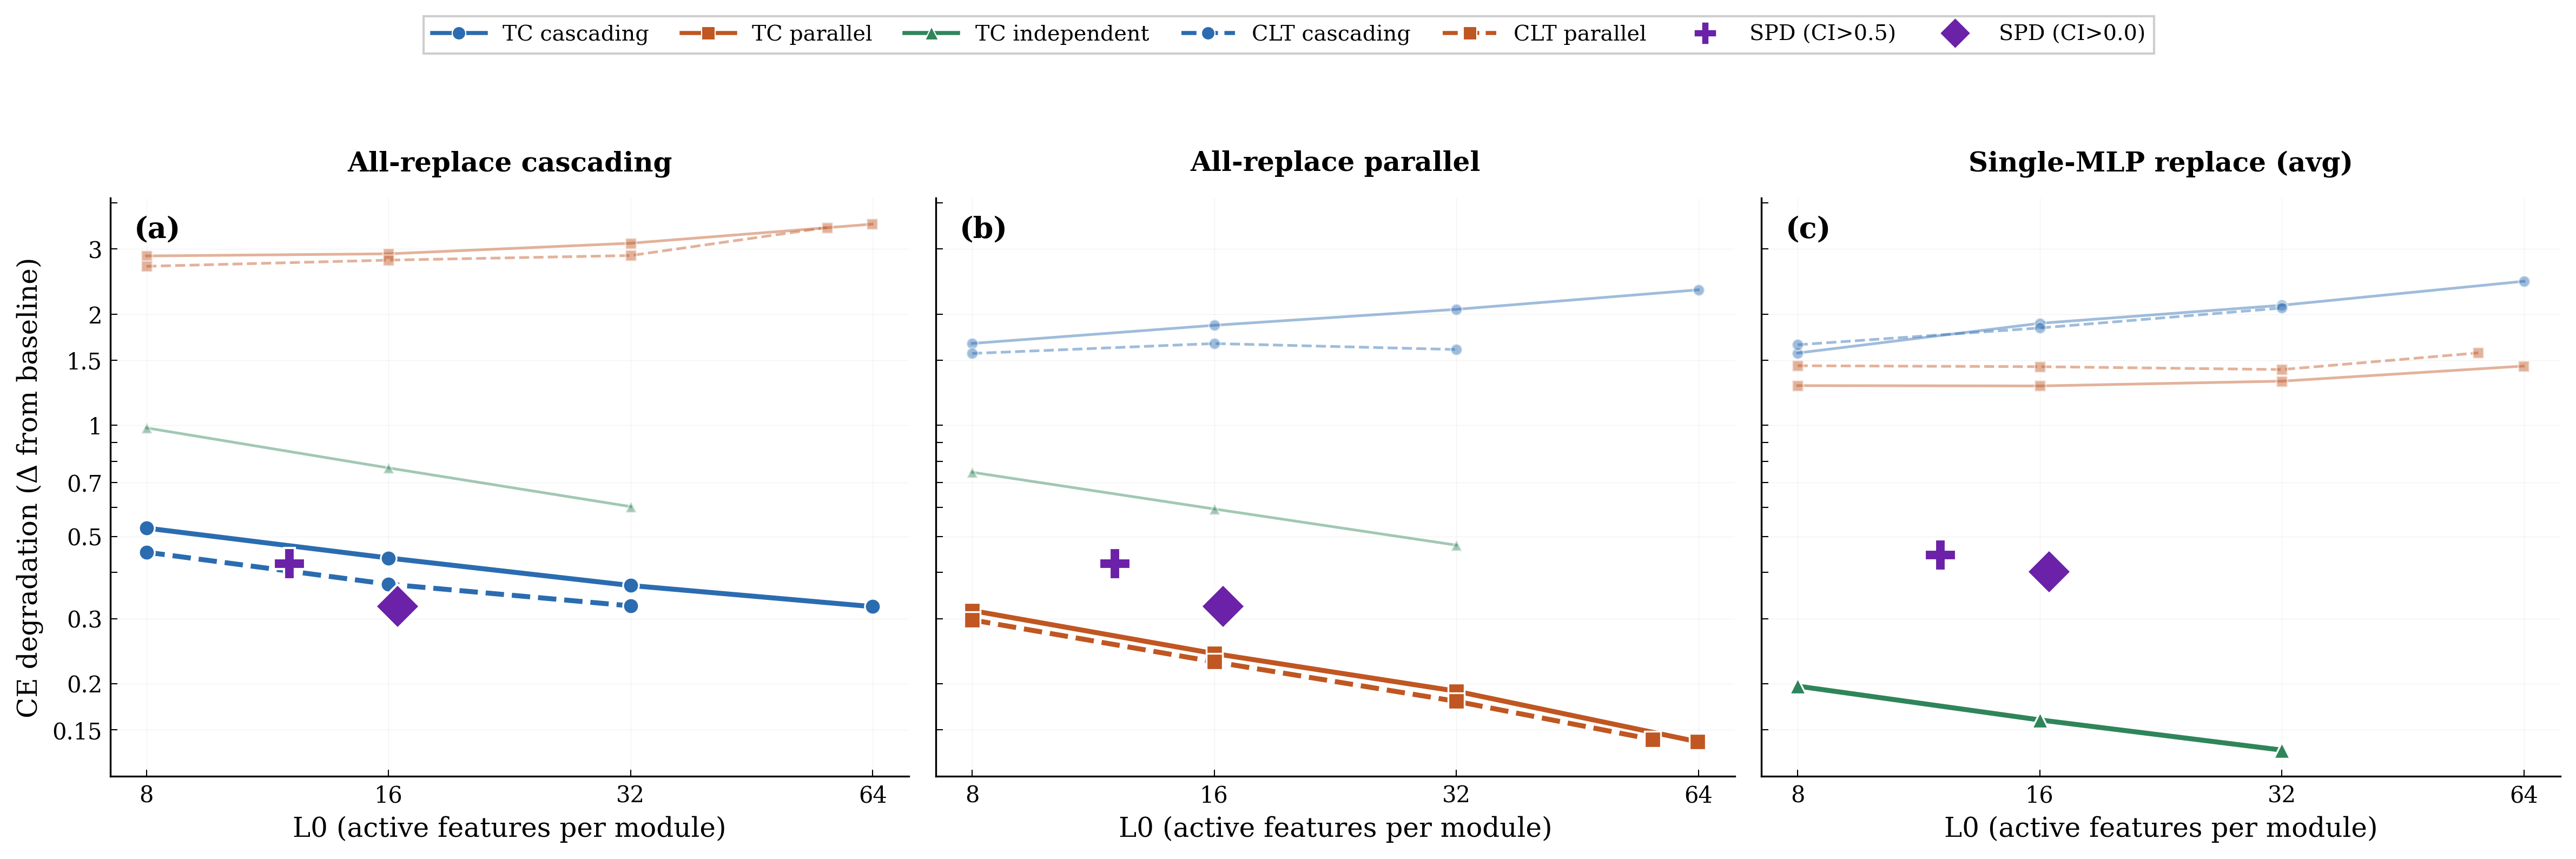
\includegraphics[width=\textwidth]{figures/eval_e2e_pareto.png}
  \caption{CE degradation ($\Delta$ from baseline, log scale) vs.\ number of active features per module (L0, log scale) for transcoders (solid lines), CLTs (dashed lines), and VPD (markers). Each panel shows a different evaluation mode: \textbf{(a)} all-replace cascading, \textbf{(b)} all-replace parallel, \textbf{(c)} single-MLP replace (average). Models trained in the matched mode for each panel are shown with thicker lines. VPD achieves competitive CE degradation at moderate sparsity and, unlike activation-based methods, does not degrade catastrophically under evaluation mode mismatch.}
  \label{fig:pareto-comparison}
\end{figure}

\begin{table}[t]
  \caption{CE degradation ($\Delta$) from baseline (CE $= 2.91$) for all methods and evaluation modes. Bold values indicate the matched evaluation mode for each training strategy. VPD results are shown at two causal importance thresholds.}
  \label{tab:pareto-results}
  \centering
  \small
  \begin{tabular}{llrrrr}
    \toprule
    \textbf{Model} & \textbf{Training mode} & \textbf{L0} & \textbf{Cascading $\Delta$} & \textbf{Parallel $\Delta$} & \textbf{Single $\Delta$} \\
    \midrule
    TC  & Cascading   &  8.0 & \textbf{0.53} & 1.67 & 1.57 \\
    TC  & Cascading   & 16.0 & \textbf{0.44} & 1.87 & 1.89 \\
    TC  & Cascading   & 32.0 & \textbf{0.37} & 2.06 & 2.11 \\
    TC  & Cascading   & 64.0 & \textbf{0.32} & 2.33 & 2.45 \\
    \midrule
    TC  & Parallel    &  8.0 & 2.87 & \textbf{0.32} & 1.28 \\
    TC  & Parallel    & 16.0 & 2.91 & \textbf{0.24} & 1.28 \\
    TC  & Parallel    & 32.0 & 3.11 & \textbf{0.19} & 1.32 \\
    TC  & Parallel    & 64.0 & 3.50 & \textbf{0.14} & 1.45 \\
    \midrule
    TC  & Independent &  8.0 & 0.98 & 0.75 & \textbf{0.20} \\
    TC  & Independent & 16.0 & 0.77 & 0.59 & \textbf{0.16} \\
    TC  & Independent & 32.0 & 0.60 & 0.47 & \textbf{0.13} \\
    \midrule
    CLT & Cascading   &  8.0 & \textbf{0.45} & 1.57 & 1.65 \\
    CLT & Cascading   & 16.0 & \textbf{0.37} & 1.67 & 1.83 \\
    CLT & Cascading   & 32.0 & \textbf{0.32} & 1.60 & 2.08 \\
    \midrule
    CLT & Parallel    &  8.0 & 2.69 & \textbf{0.30} & 1.45 \\
    CLT & Parallel    & 16.0 & 2.80 & \textbf{0.23} & 1.44 \\
    CLT & Parallel    & 32.0 & 2.88 & \textbf{0.18} & 1.42 \\
    CLT & Parallel    & 64.0 & 3.43 & \textbf{0.14} & 1.57 \\
    \midrule
    VPD & CI $> 0.5$  & 12.0 & ---           & 0.42 & 0.45 \\
    VPD & CI $> 0.0$  & 16.4 & ---           & 0.32 & 0.40 \\
    \bottomrule
  \end{tabular}
\end{table}
